\chapter{Data analysis and preprocessing}\label{data}

Our data comprises approximately 400 sessions collected from 80 patients. These
sessions were recorded at various time points and are not uniformly spaced.
Each session's data includes a 3D scan of the patient, along with several
measurements such as weight, height, body fat percentage, etc.

\begin{table}[h]
    \centering
    \begin{tabular}{c c l c}
        \toprule
        Type                               & Source                                                                                         & Measurement (unit)                        \\
        \midrule
        \multirow{3}{*}{Anthropometric}    & \multirow{3}{4cm}{flexible measuring tape}                                                     & Wrist (cm) (kg)                           \\
                                           &                                                                                                & Waist (cm)                                \\
                                           &                                                                                                & Hip (cm)                                  \\
        \midrule

        \multirow{6}{*}{Body composition}  & \multirow{6}{4cm}{Tanita\textregistered\ MC 780-P MA and Seca\textregistered\ 213 stadiometer} & Fat per limb and trunk (\%)               \\
                                           &                                                                                                & Muscle per limb and trunk (\%)            \\
                                           &                                                                                                & Total fat and muscle (\%)                 \\
                                           &                                                                                                & Visceral fat area (cm\textsuperscript{2}) \\
                                           &                                                                                                & Weight (kg)                               \\
                                           &                                                                                                & Height (m)                                \\
        \midrule

        \multirow{3}{*}{Other, Lifestyle}  & \multirow{3}{4cm}{Interview}                                                                   & Activity   (score)                        \\
                                           &                                                                                                & Gender                                    \\
                                           &                                                                                                & Age (years)                               \\

        \midrule

        \multirow{3}{*}{Blood (capillary)} & \multirow{3}{4cm}{Accutrend\textregistered\ Plus}                                              & Glucose (mg/dL)                           \\
                                           &                                                                                                & Cholesterol (mg/dL)                       \\
                                           &                                                                                                & Triglycerides (mg/dL)                     \\

        \midrule

        \multirow{2}{*}{Blood pressure}    & \multirow{2}{4cm}{Omron\textregistered\ M3}                                                    & Systolic pressure (mmHg)                  \\
                                           &

                                           & Diastolic pressure (mmHg)                                                                                                                  \\
        \bottomrule

    \end{tabular}
    \caption{Measurements collected from each session.}
\end{table}

\todo[]{${https://rua.ua.es/dspace/bitstream/10045/124160/6/Garcia-dUrso_etal_2022_IEEEAccess.pdf}$}

However, the data requires cleaning before usage. Some sessions lack certain
measurements, and there are numerous outliers within the data. After cleaning,
we utilized about 200 sessions.

\subsection{Data cleaning}

We developed a data cleaning pipeline using the \gls{pandas} library. This
pipeline fixes some errors in the data, removes outliers and sessions with
missing measurements.

\section{Body representation}

In order to represent the body shape we opted to use \gls{smpl}. \gls{smpl}
encodes the body shape and pose using a low-dimensional linear space. The body
shape is encoded using 10 shape parameters ($\beta$), and the pose is encoded
using 72 pose parameters ($\theta$). As our interest lies in body shape, we
employed only the shape parameters.

We extracted \gls{smpl} parameters --- shape ($\beta$) and pose ($\theta$) ---
from the 3D scans using a custom minimization algorithm.

\def\betaVar{3}
\def\imgWidth{0.3\textwidth}
\def\betaWidth{\textwidth}

\begin{figure}[ht!]
    \centering
    \begin{minipage}[b]{\textwidth}
        \centering
        \includegraphics[width=\imgWidth]{files/visualize_betas/beta_0_-\betaVar_m}
        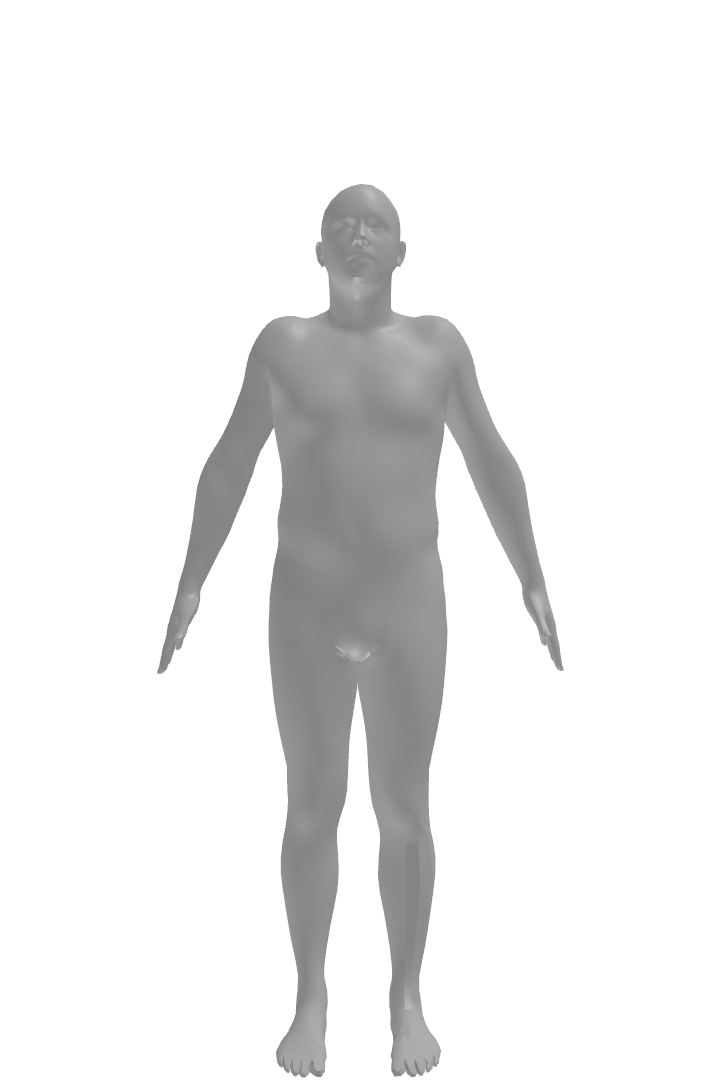
\includegraphics[width=\imgWidth]{files/visualize_betas/baseline_m}
        \includegraphics[width=\imgWidth]{files/visualize_betas/beta_0_\betaVar_m}
        \linebreak
        \includegraphics[width=\imgWidth]{files/visualize_betas/beta_0_-\betaVar_f}
        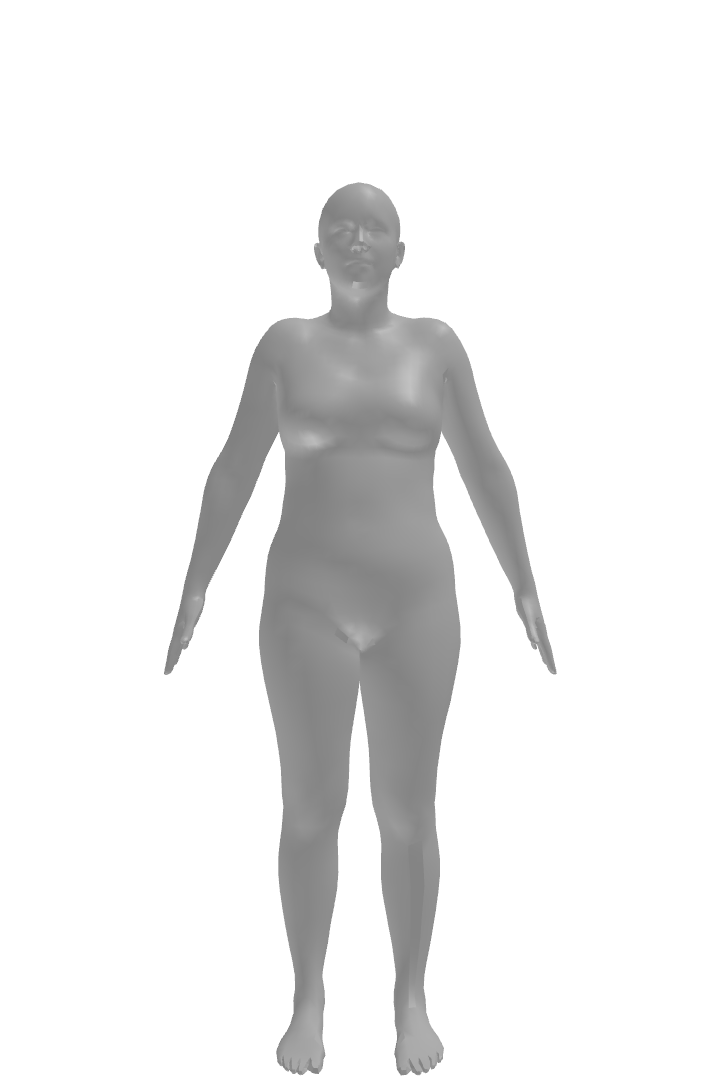
\includegraphics[width=\imgWidth]{files/visualize_betas/baseline_f}
        \includegraphics[width=\imgWidth]{files/visualize_betas/beta_0_\betaVar_f}
        \caption[Effect of varying $\beta_1$ in SMPL.]{$\beta_1 = [-\betaVar, 0, +\betaVar]$.}
        \label{fig:beta-1-vis}
    \end{minipage}
\end{figure}

\begin{figure}[ht!]
    \centering

    \begin{minipage}[b]{\textwidth}
        \centering
        \includegraphics[width=\imgWidth]{files/visualize_betas/beta_1_-\betaVar_m}
        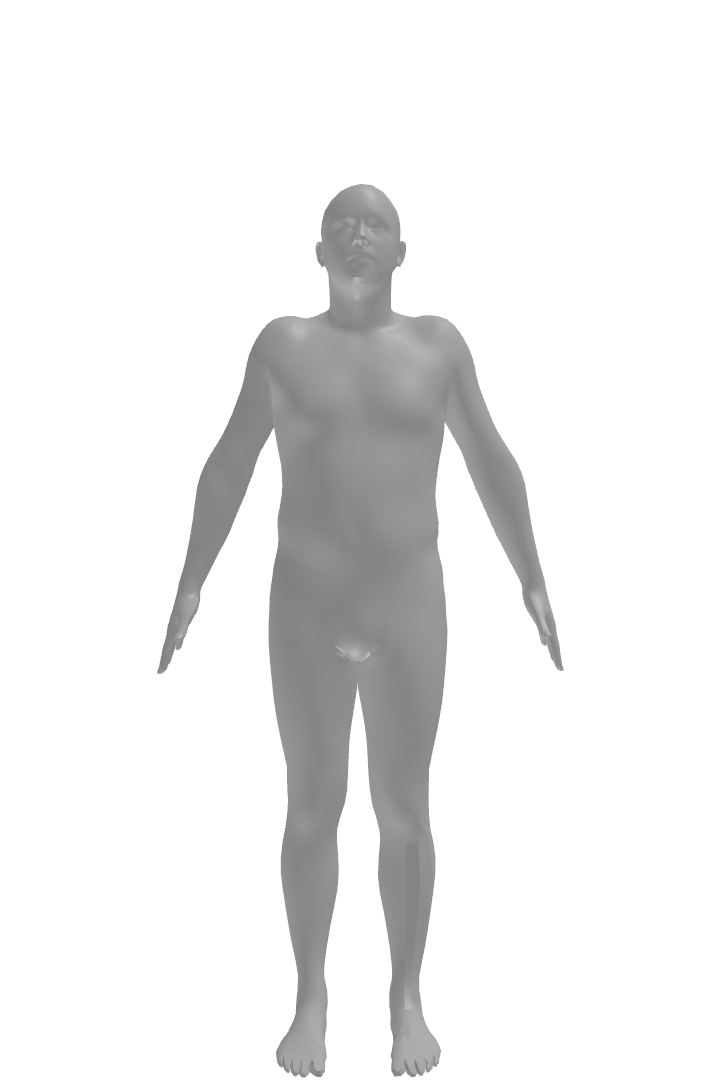
\includegraphics[width=\imgWidth]{files/visualize_betas/baseline_m}
        \includegraphics[width=\imgWidth]{files/visualize_betas/beta_1_\betaVar_m}
        \linebreak
        \includegraphics[width=\imgWidth]{files/visualize_betas/beta_1_-\betaVar_f}
        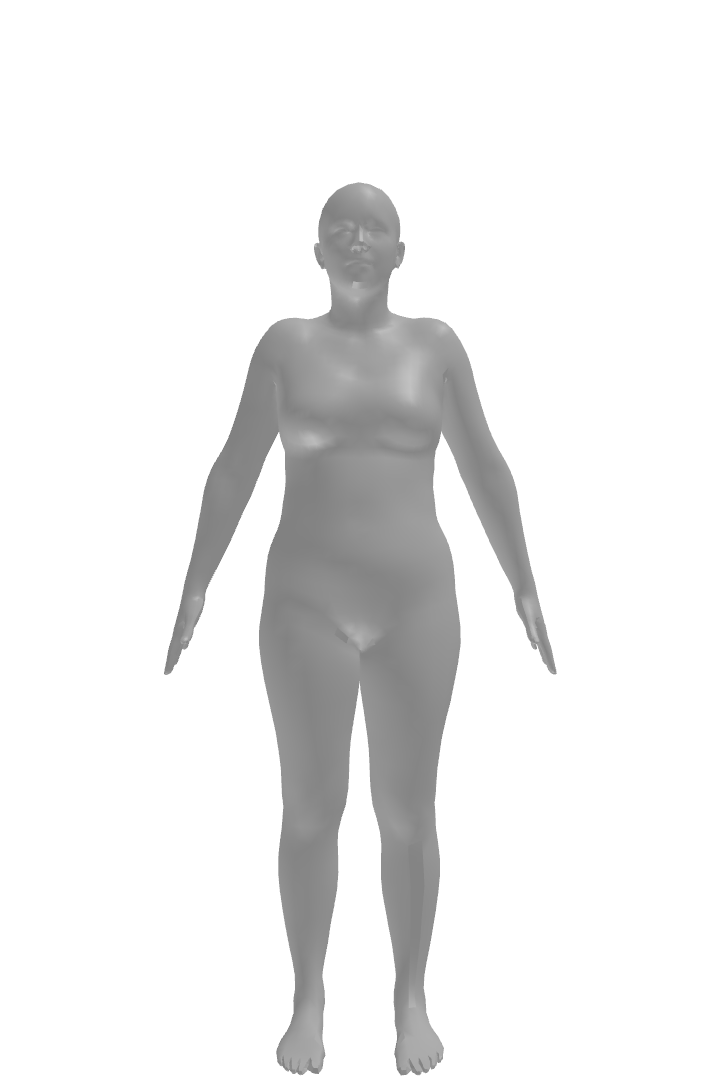
\includegraphics[width=\imgWidth]{files/visualize_betas/baseline_f}
        \includegraphics[width=\imgWidth]{files/visualize_betas/beta_1_\betaVar_f}
        \caption[Effect of varying $\beta_2$ in SMPL.]{$\beta_2 = [-\betaVar, 0, +\betaVar]$.}
    \end{minipage}
\end{figure}

\begin{figure}[ht!]
    \centering

    \begin{minipage}[b]{\textwidth}
        \centering
        \includegraphics[width=\imgWidth]{files/visualize_betas/beta_2_-\betaVar_m}
        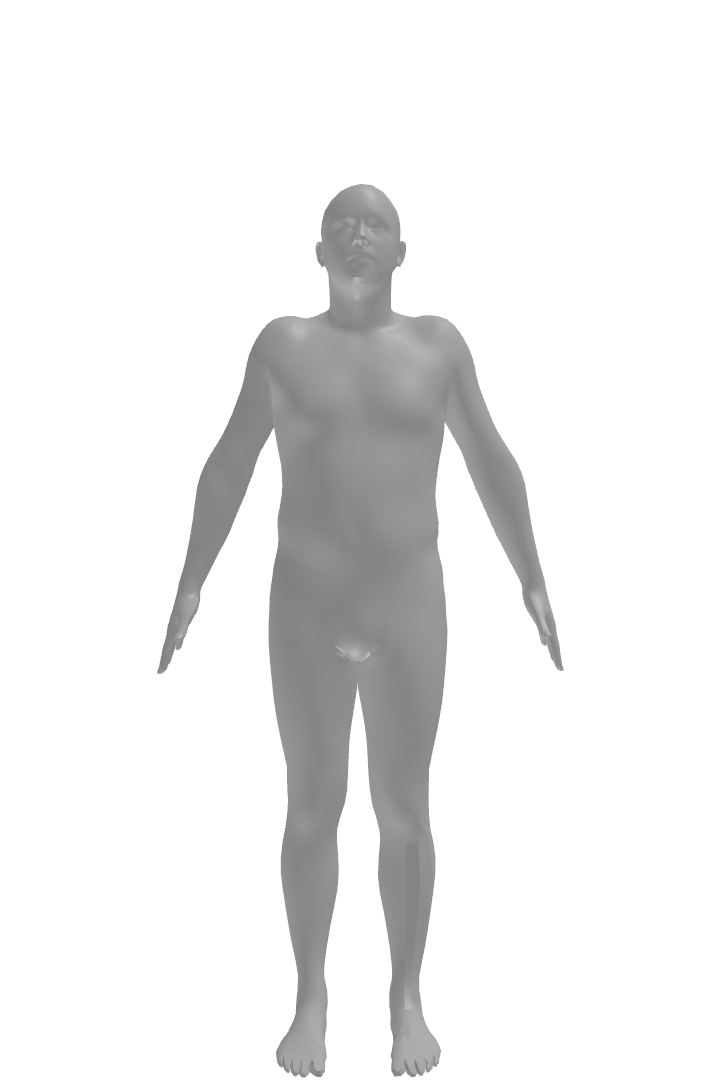
\includegraphics[width=\imgWidth]{files/visualize_betas/baseline_m}
        \includegraphics[width=\imgWidth]{files/visualize_betas/beta_2_\betaVar_m}
        \linebreak
        \includegraphics[width=\imgWidth]{files/visualize_betas/beta_2_-\betaVar_f}
        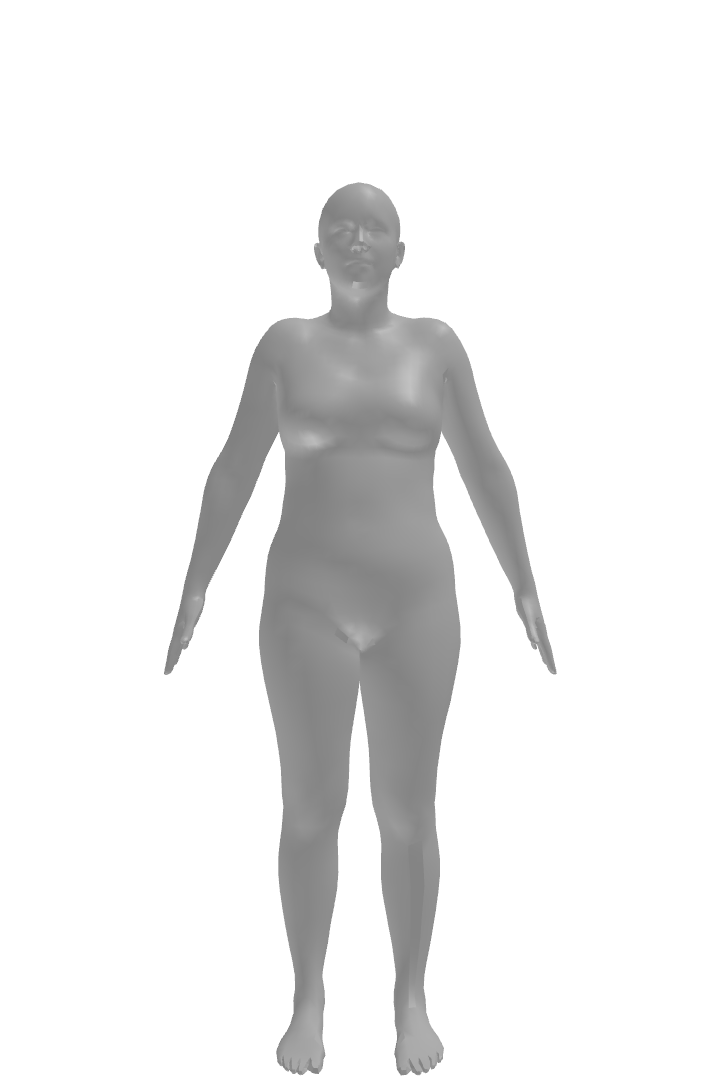
\includegraphics[width=\imgWidth]{files/visualize_betas/baseline_f}
        \includegraphics[width=\imgWidth]{files/visualize_betas/beta_2_\betaVar_f}
        \caption[Effect of varying $\beta_3$ in SMPL.]{$\beta_3 = [-\betaVar, 0, +\betaVar]$.}
    \end{minipage}
\end{figure}

\begin{figure}[ht!]
    \centering

    \begin{minipage}[b]{\textwidth}
        \centering
        \includegraphics[width=\imgWidth]{files/visualize_betas/beta_3_-\betaVar_m}
        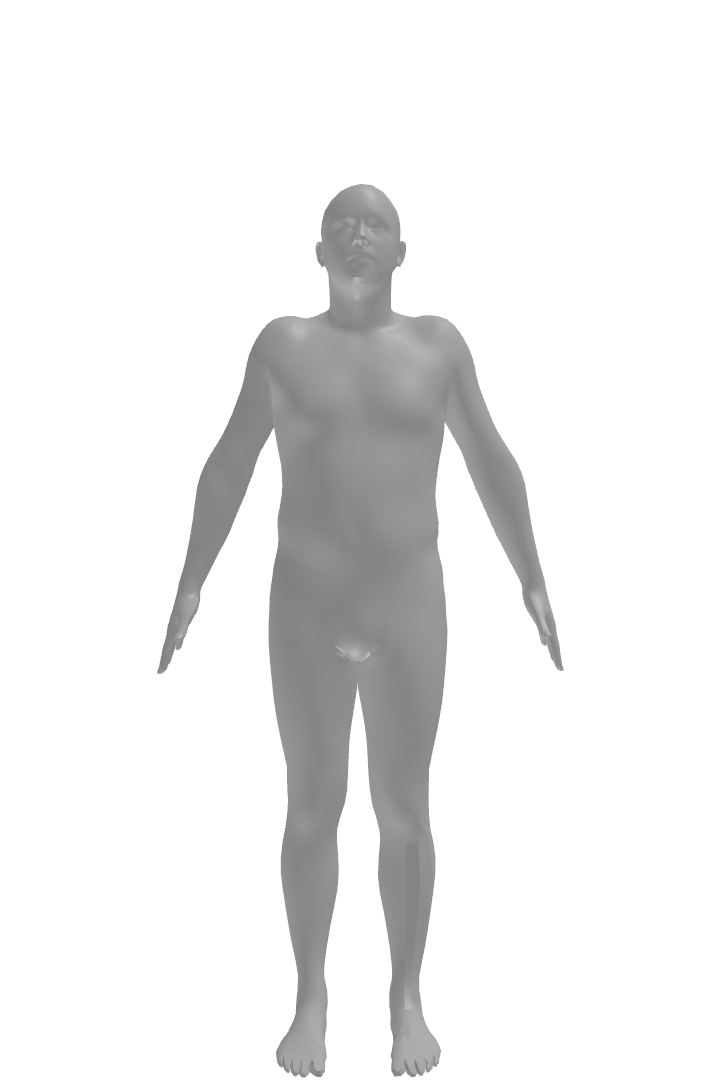
\includegraphics[width=\imgWidth]{files/visualize_betas/baseline_m}
        \includegraphics[width=\imgWidth]{files/visualize_betas/beta_3_\betaVar_m}
        \linebreak
        \includegraphics[width=\imgWidth]{files/visualize_betas/beta_3_-\betaVar_f}
        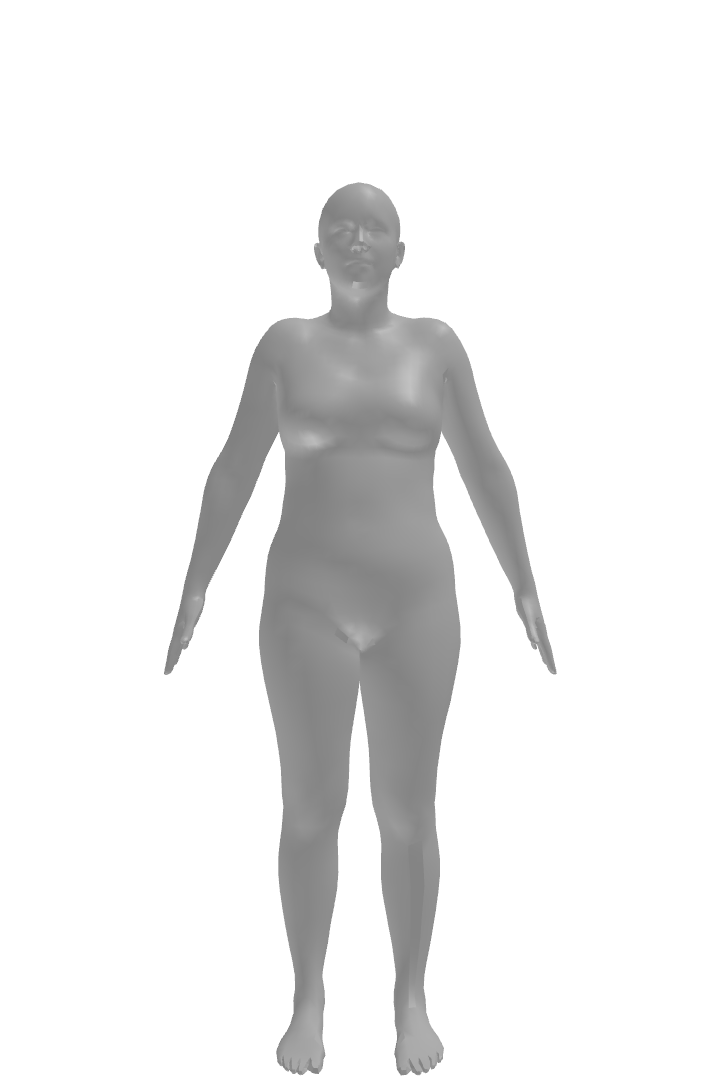
\includegraphics[width=\imgWidth]{files/visualize_betas/baseline_f}
        \includegraphics[width=\imgWidth]{files/visualize_betas/beta_3_\betaVar_f}
        \caption[Effect of varying $\beta_4$ in SMPL.]{$\beta_4 = [-\betaVar, 0, +\betaVar]$.}
    \end{minipage}
\end{figure}

\begin{figure}[ht!]
    \centering

    \begin{minipage}[b]{\textwidth}
        \centering
        \includegraphics[width=\imgWidth]{files/visualize_betas/beta_4_-\betaVar_m}
        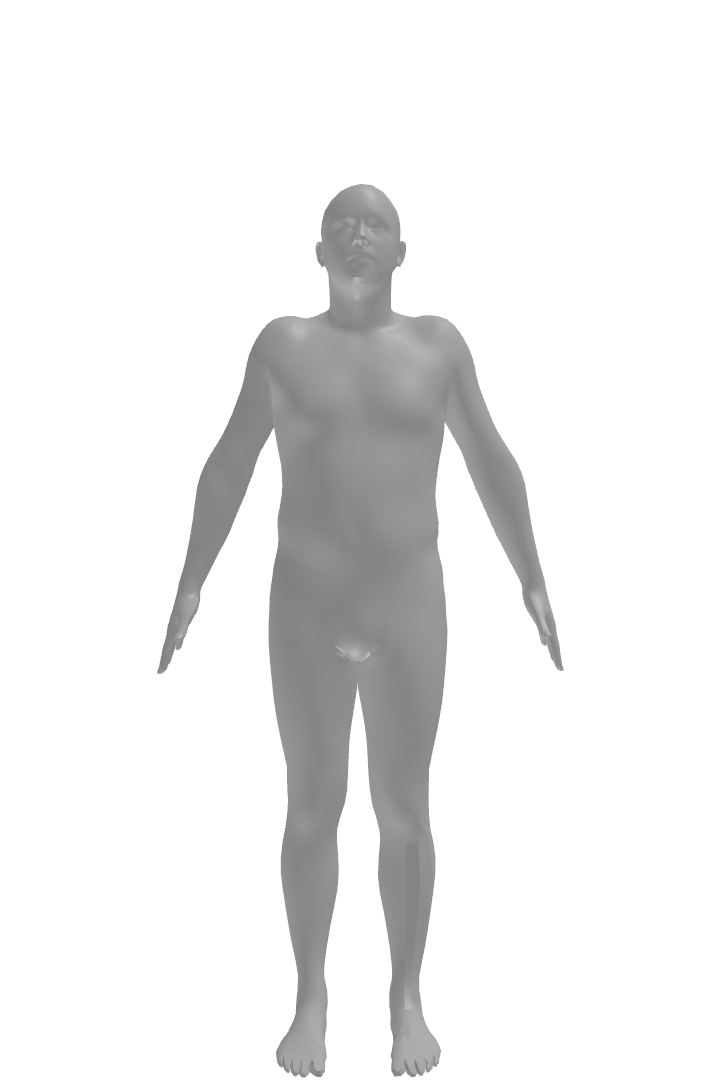
\includegraphics[width=\imgWidth]{files/visualize_betas/baseline_m}
        \includegraphics[width=\imgWidth]{files/visualize_betas/beta_4_\betaVar_m}
        \linebreak
        \includegraphics[width=\imgWidth]{files/visualize_betas/beta_4_-\betaVar_f}
        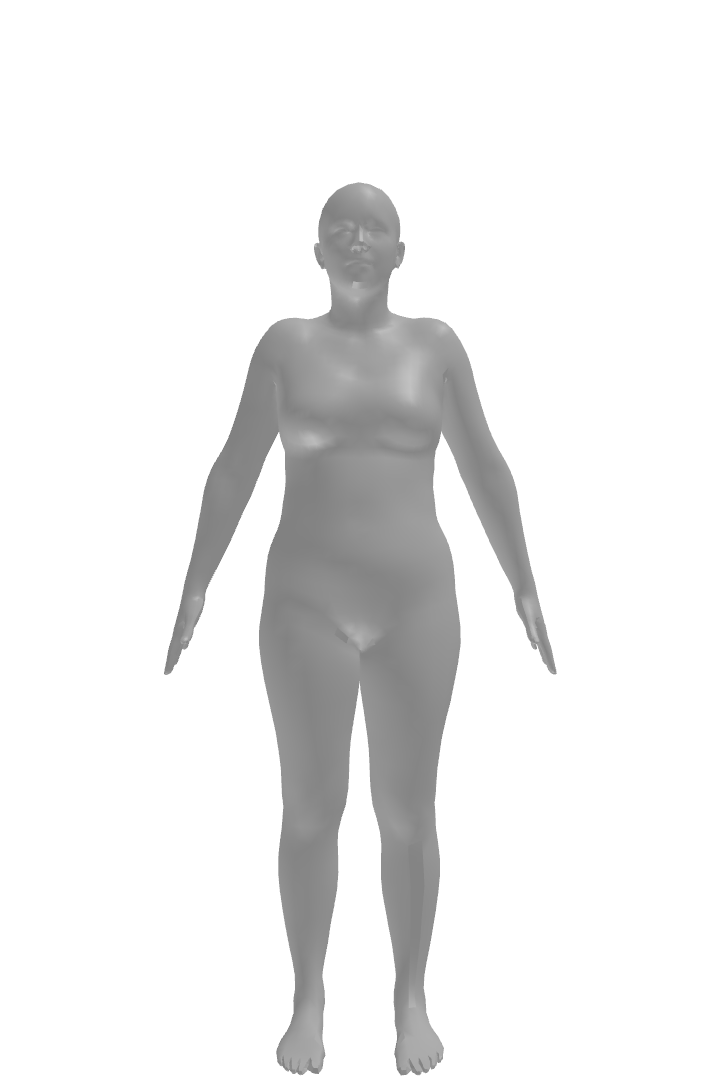
\includegraphics[width=\imgWidth]{files/visualize_betas/baseline_f}
        \includegraphics[width=\imgWidth]{files/visualize_betas/beta_4_\betaVar_f}
        \caption[Effect of varying $\beta_5$ in SMPL.]{$\beta_5 = [-\betaVar, 0, +\betaVar]$.}
    \end{minipage}
\end{figure}

\begin{figure}[ht!]
    \centering

    \begin{minipage}[b]{\textwidth}
        \centering
        \includegraphics[width=\imgWidth]{files/visualize_betas/beta_5_-\betaVar_m}
        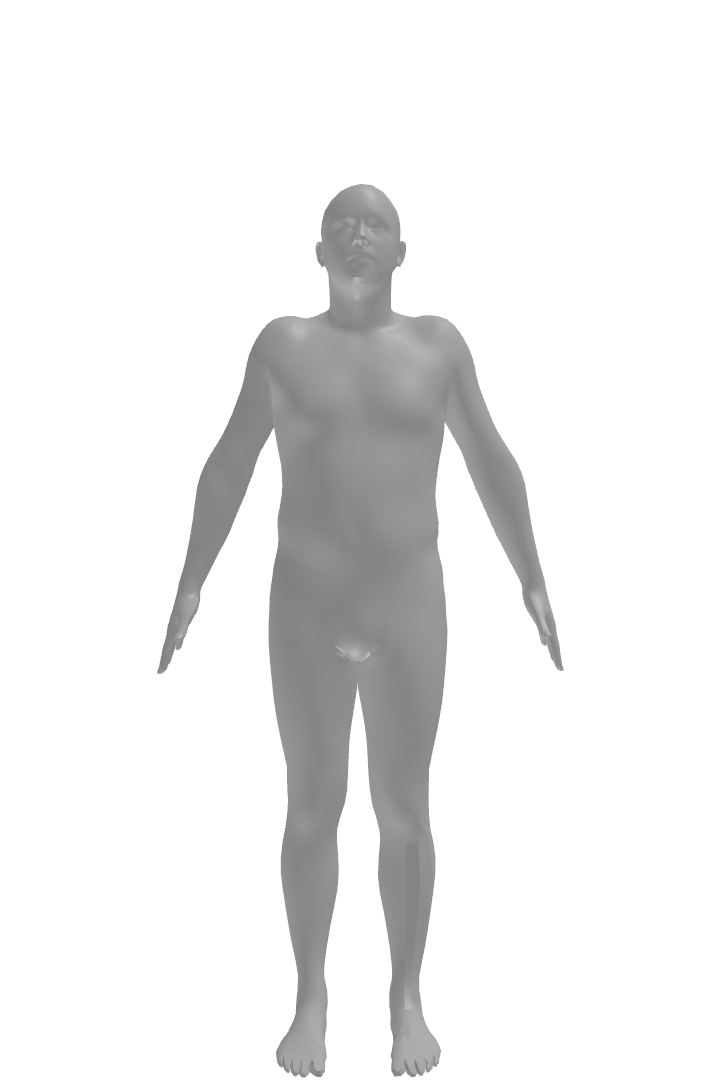
\includegraphics[width=\imgWidth]{files/visualize_betas/baseline_m}
        \includegraphics[width=\imgWidth]{files/visualize_betas/beta_5_\betaVar_m}
        \linebreak
        \includegraphics[width=\imgWidth]{files/visualize_betas/beta_5_-\betaVar_f}
        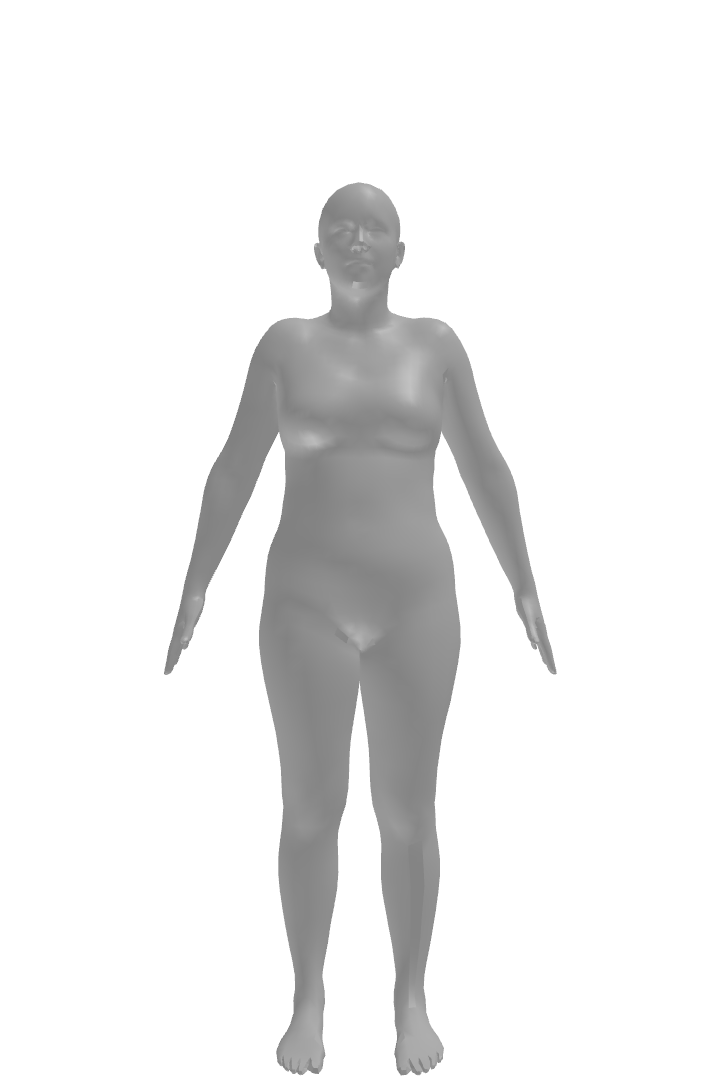
\includegraphics[width=\imgWidth]{files/visualize_betas/baseline_f}
        \includegraphics[width=\imgWidth]{files/visualize_betas/beta_5_\betaVar_f}
        \caption[Effect of varying $\beta_6$ in SMPL.]{$\beta_6 = [-\betaVar, 0, +\betaVar]$.}
    \end{minipage}
\end{figure}

\begin{figure}[ht!]
    \centering

    \begin{minipage}[b]{\textwidth}
        \centering
        \includegraphics[width=\imgWidth]{files/visualize_betas/beta_6_-\betaVar_m}
        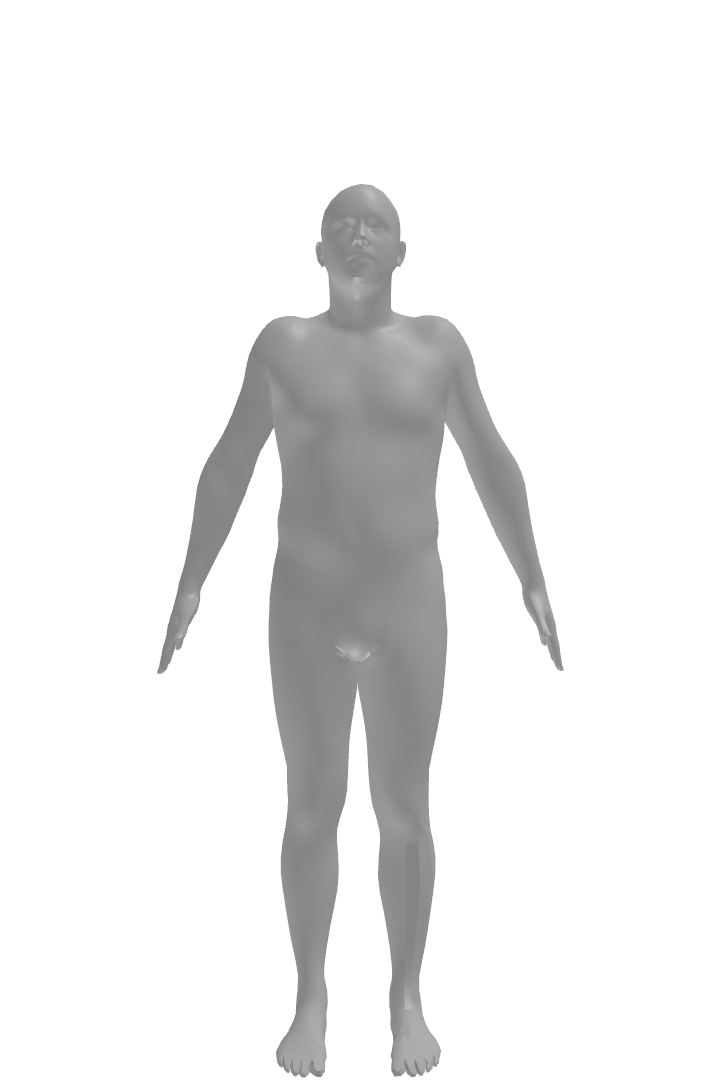
\includegraphics[width=\imgWidth]{files/visualize_betas/baseline_m}
        \includegraphics[width=\imgWidth]{files/visualize_betas/beta_6_\betaVar_m}
        \linebreak
        \includegraphics[width=\imgWidth]{files/visualize_betas/beta_6_-\betaVar_f}
        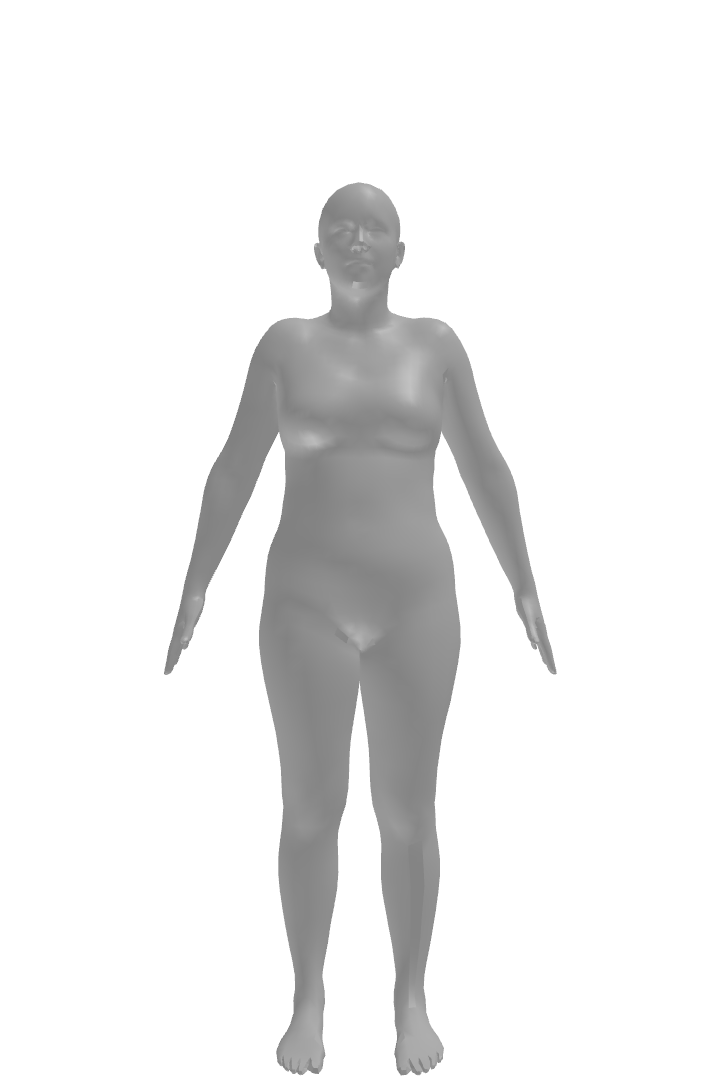
\includegraphics[width=\imgWidth]{files/visualize_betas/baseline_f}
        \includegraphics[width=\imgWidth]{files/visualize_betas/beta_6_\betaVar_f}
        \caption[Effect of varying $\beta_7$ in SMPL.]{$\beta_7 = [-\betaVar, 0, +\betaVar]$.}
    \end{minipage}
\end{figure}

\begin{figure}[ht!]
    \centering

    \begin{minipage}[b]{\textwidth}
        \centering
        \includegraphics[width=\imgWidth]{files/visualize_betas/beta_7_-\betaVar_m}
        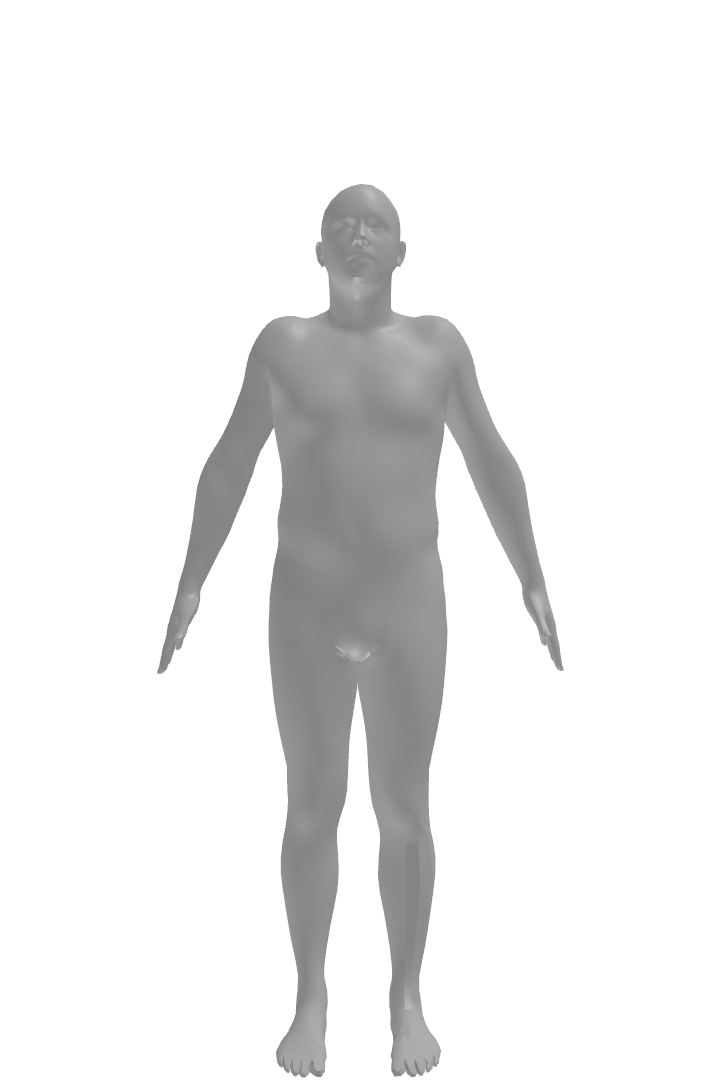
\includegraphics[width=\imgWidth]{files/visualize_betas/baseline_m}
        \includegraphics[width=\imgWidth]{files/visualize_betas/beta_7_\betaVar_m}
        \linebreak
        \includegraphics[width=\imgWidth]{files/visualize_betas/beta_7_-\betaVar_f}
        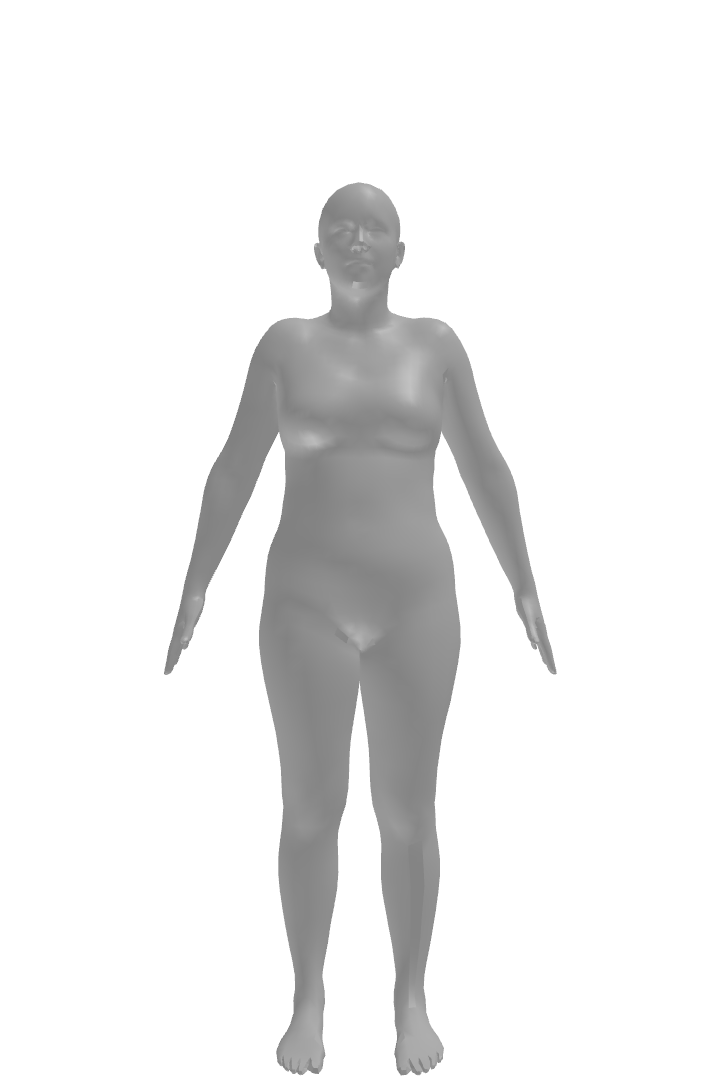
\includegraphics[width=\imgWidth]{files/visualize_betas/baseline_f}
        \includegraphics[width=\imgWidth]{files/visualize_betas/beta_7_\betaVar_f}
        \caption[Effect of varying $\beta_8$ in SMPL.]{$\beta_8 = [-\betaVar, 0, +\betaVar]$.}
    \end{minipage}
\end{figure}

\begin{figure}[ht!]
    \centering

    \begin{minipage}[b]{\textwidth}
        \centering
        \includegraphics[width=\imgWidth]{files/visualize_betas/beta_8_-\betaVar_m}
        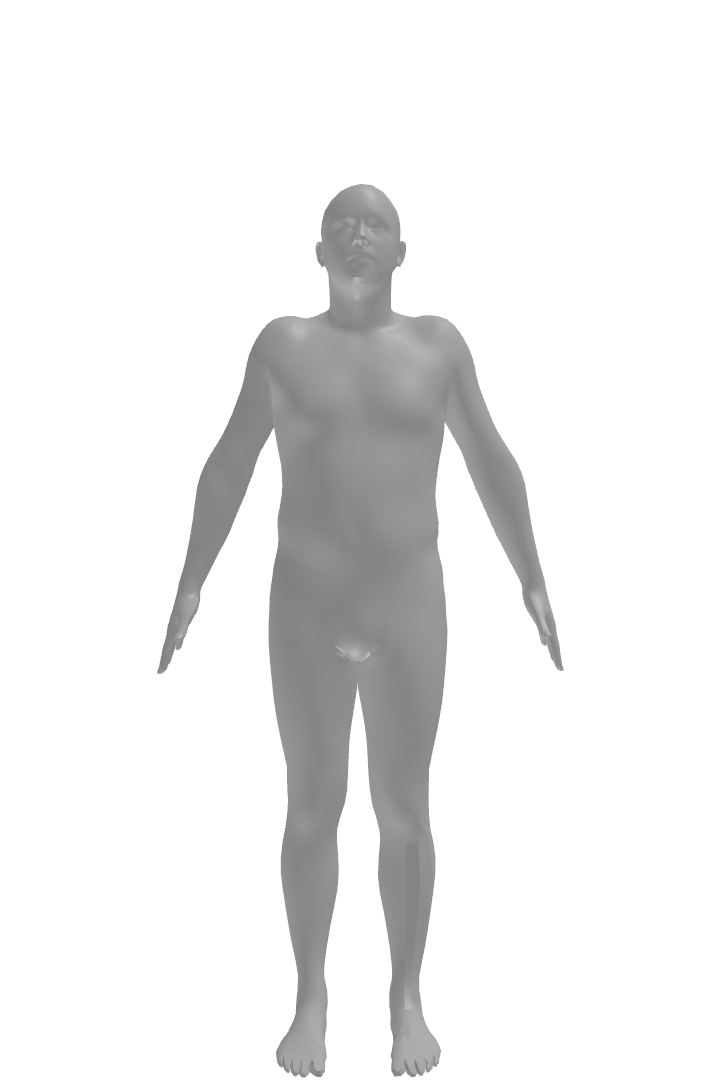
\includegraphics[width=\imgWidth]{files/visualize_betas/baseline_m}
        \includegraphics[width=\imgWidth]{files/visualize_betas/beta_8_\betaVar_m}
        \linebreak
        \includegraphics[width=\imgWidth]{files/visualize_betas/beta_8_-\betaVar_f}
        \includegraphics[width=\imgWidth]{files/visualize_betas/baseline_f}
        \includegraphics[width=\imgWidth]{files/visualize_betas/beta_8_\betaVar_f}
        \caption[Effect of varying $\beta_9$ in SMPL.]{$\beta_9 = [-\betaVar, 0, +\betaVar]$.}
    \end{minipage}
\end{figure}

\begin{figure}[ht!]
    \centering

    \begin{minipage}[b]{\textwidth}
        \centering
        \includegraphics[width=\imgWidth]{files/visualize_betas/beta_9_-\betaVar_m}
        \includegraphics[width=\imgWidth]{files/visualize_betas/baseline_m}
        \includegraphics[width=\imgWidth]{files/visualize_betas/beta_9_\betaVar_m}
        \linebreak
        \includegraphics[width=\imgWidth]{files/visualize_betas/beta_9_-\betaVar_f}
        \includegraphics[width=\imgWidth]{files/visualize_betas/baseline_f}
        \includegraphics[width=\imgWidth]{files/visualize_betas/beta_9_\betaVar_f}
        \caption[Effect of varying $\beta_{10}$ in SMPL.]{$\beta_{10} = [-\betaVar, 0, +\betaVar]$.}
        \label{fig:beta-10-vis}
    \end{minipage}
\end{figure}


Figure~\ref{fig:beta-vis} shows the effect of varying the shape parameters. We
have used a scale of 3 to better show their effect, but in practice the values
are much smaller. $\beta_0$ controls the overall height of the body, while
$\beta_1$ has a large correlation with the body mass index.

\begin{table}[h]
    \centering
    \begin{tabular}{c | c c c c c c c c c c}
        \toprule
             & $\beta_1$ & $\beta_2$ & $\beta_3$ & $\beta_4$ & $\beta_5$ & $\beta_6$ & $\beta_7$ & $\beta_8$ & $\beta_9$ & $\beta_{10}$ \\
        \midrule
        mean & 0.88      & -0.73     & 0.34      & 0.01      & 0.06      & 0.06      & 0.11      & 0.02      & 0.01      & 0.11         \\

        std  & 0.97      & 0.78      & 0.26      & 0.21      & 0.12      & 0.13      & 0.08      & 0.03      & 0.03      & 0.08         \\

        min  & -1.42     & -2.57     & -0.64     & -0.65     & -0.23     & -0.25     & -0.14     & -0.07     & -0.08     &
        -0.17                                                                                                                           \\

        25\% & 0.12      & -1.26     & 0.15      & -0.14     & -0.01     & -0.02     & 0.04      & 0.00      & -0.01     & 0.06         \\

        50\% & 0.94      & -0.69     & 0.36      & 0.03      & 0.04      & 0.02      & 0.11      & 0.02      & 0.01      & 0.11         \\

        75\% & 1.66      & -0.20     & 0.52      & 0.17      & 0.14      & 0.14      & 0.16      & 0.04      & 0.04      & 0.17         \\

        max  & 2.90      & 2.96      & 0.97      & 0.45      & 0.39      & 0.47      & 0.36      & 0.13      & 0.16      & 0.30         \\
        \bottomrule
    \end{tabular}
    \caption{Statistics of the shape parameters}
\end{table}